\RequirePackage{pdf14}
% ===============================================================================
% = LaTeX Beamer Template des Arbeitsbereichs Sicherheit in verteilten Systemem
% = (c) 2012 Prof. Dr. Hannes Federrath, Uni Hamburg, Fachbereich Informatik
% = http://www.informatik.uni-hamburg.de/svs/
% ===============================================================================
%
\documentclass[t]{beamer} 
% Option t              Place text of slides at the (vertical) top of the slides.
% Option handout        Ein PDF ohne Pausen und Overlayeffekte erzeugen.
% Option aspectratio=43 169 => 16:9, 1610 => 16:10, 43 => 4:3
\usepackage[utf8]{inputenc}
\usepackage[ngerman]{babel}
\usepackage{graphicx,xcolor}
\usepackage[T1]{fontenc} % 8-Bit-Zeichen; ermöglicht korrektes Kopieren von Umlauten aus dem pdf 
\usepackage[scaled]{helvet}
\usepackage{ulem}
\usepackage{pdfpages}

\usepackage{beamerthemedefault}

% Ränder definieren
\setbeamersize{text margin left=5ex, text margin right=5ex}

% Farbdefinitionen
\definecolor{svsgrau1}{RGB}{191,191,191} % Balken in Kopfzeile
\definecolor{svsgrau2}{RGB}{123,123,123} % Folienüberschriften
\definecolor{svsrot}{RGB}{255,0,0} % Bullets
\definecolor{svshellblau1}{RGB}{153,204,255} % Block Hintergrund
\definecolor{svshellblau2}{RGB}{24,113,248} % Anstrich Ebene 2
\definecolor{svsdunkelblau}{RGB}{38,82,128} % Text der Ebene 1

% Navigationsleiste ausblenden
\beamertemplatenavigationsymbolsempty 

% Farben der Bullets der Ebenen
\setbeamercolor{itemize item}{fg=svsrot}
\setbeamercolor{itemize subitem}{fg=svshellblau2}
\setbeamercolor{enumerate item}{parent=itemize item}
\setbeamercolor{enumerate subitem}{parent=itemize subitem}

% Formen der Bullets der Ebenen
\setbeamertemplate{itemize item}[circle] 
\setbeamertemplate{itemize subitem}{--} 
\setbeamertemplate{itemize subsubitem}[circle] 

% Farben der Texte 
\setbeamercolor{title}{fg=black}
\setbeamercolor{structure}{fg=svsgrau2}
\setbeamercolor{section in toc}{fg=black}
\setbeamercolor{framesubtitle}{fg=svsdunkelblau}
\setbeamercolor{itemize/enumerate body}{fg=svsdunkelblau}
\setbeamercolor{itemize/enumerate subbody}{fg=black}
\setbeamercolor{itemize/enumerate subsubbody}{fg=black}

% Zeichensätze der Texte
\setbeamerfont{author}{size=\normalsize}
\setbeamerfont{institute}{size=\normalsize}
\setbeamerfont{date}{size=\normalsize}
\setbeamerfont{frametitle}{size=\large}
\setbeamerfont{framesubtitle}{size=\footnotesize\raggedleft}
\setbeamerfont{sections/subsections in toc}{size=\normalsize}
\setbeamerfont{itemize/enumerate body}{size=\normalsize}
\setbeamerfont{itemize/enumerate subbody}{size=\normalsize}
\setbeamerfont{itemize/enumerate subsubbody}{size=\normalsize}

% Definitionen für farbig hinterlegten Block 
\setbeamertemplate{blocks}[rounded]
\setbeamercolor{block title}{fg=black,bg=svshellblau1}
\setbeamercolor{block body}{parent=normal text,use=block title,bg=block title.bg!25!bg}
\setbeamerfont{block title}{size=\normalsize}
\setbeamerfont{block body}{size=\normalsize}

% Definitionen für Agenda (FIXME: noch stärker an normale Listendefs. anpassen)
\setbeamertemplate{section in toc}[sections numbered]
\setbeamertemplate{subsection in toc}[square]

% Kopfzeile
\setbeamertemplate{headline}{
	\includegraphics[height=8mm]{pic/UHH-Logo_2010_ohneText.png}%
	\color{svsgrau1}\rule{\paperwidth}{8mm}\newline
	\mbox{}\rule{1em}{0pt}\rule{0pt}{8ex}
	\dotfill\newline\vspace{-7.3ex}
}

% Fusszeile
\setbeamertemplate{footline}[text line]{
	\parbox[b]{50mm}{\insertframenumber\\[1ex]}
}

% Hintergrund Titelseite
\defbeamertemplate{background canvas}{titlepage}{%
	{\color{svsgrau1}\vrule width\paperwidth height0.7\paperheight}%
	{\color{white}\vrule width\paperwidth height0.3\paperheight}%
}

% =============================
% = Ab hier Inhalte ändern... 
% =============================

\title{IPsec und die NSA}
\author[Eris, Martens, Scholz]{Mustafa Eris, Jim Martens, Benjamin Scholz}
\institute[Uni Hamburg]{Universität Hamburg\\ Fachbereich Informatik}
\date{27.01.2015}

\begin{document}

\begingroup
	\setbeamertemplate{background canvas}[titlepage]
	\begin{frame}[plain]
		\vskip8mm
		\includegraphics[width=2.2cm]{pic/svs_logo_hires-ohne-was.png}
		\vskip-20mm % dies geht nur bei kurzen Vortragstiteln
		\titlepage
		\vspace{\fill}
		\includegraphics[width=2.9cm]{pic/UHH-Logo_2010_Farbe_RGB_hires_nomargin.png}
		\vskip20pt
	\end{frame}
\endgroup

\begin{frame}{Agenda}
	\tableofcontents
\end{frame}

\section{Grundlagen von VPNs}
\begin{frame}
	\frametitle{Grundlagen von VPNs}
	\begin{itemize}
		\vfill
		\item VPN \(\widehat{=}\) Virtual Private Network
		\vfill
		\item gesicherte Verbindung durch unsichere Umgebung ("`Tunnel"')
		\vfill
		\item Sichere Verbindung zu lokalem Netzwerk über das Internet
		\vfill
		\item Vorteile eines privaten Netwerkes über das Internet
		\vfill
	\end{itemize}
\end{frame}

\section{VPN-Varianten}
\begin{frame}
	\frametitle{VPN-Varianten}
	\vfill
	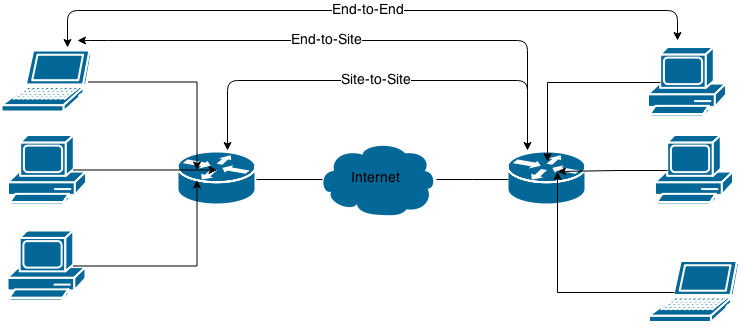
\includegraphics[width=1\textwidth]{pic/ipsec.png}
\end{frame}

\section{Anwendung}
\begin{frame}
	\frametitle{Anwendung}
	\begin{itemize}
		\vfill
		\item Zugriff auf den Arbeitsplatz
		\vfill
		\item Uni
		\vfill
		\item Umgehen von Sperren
		\vfill
		\item Youtube/Netflix
	\end{itemize}
\end{frame}

\section{NSA's War on Terror}
\begin{frame}
	\frametitle{NSA's War on Terror}
	\begin{itemize}
		\item massenweise Überwachung von unschuldigen Zivilisten
		\item absichtliche Schwächung von kryptographischen Standards
		\item Macht über die Daten von Milliarden von Menschen
		\item Macht über das Leben von Milliarden von Menschen
	\end{itemize}

	\only<1>{\(\Rightarrow\) Menschen leben in ständiger Angst, ob der potentiellen Bedrohung}
	\only<2->{\(\Rightarrow\) \sout{Menschen leben in ständiger Angst, ob der potentiellen Bedrohung}}
	
	\only<3>{\(\Rightarrow\) noch mehr Überwachung nötig, um Terror zu bekämpfen}
\end{frame}

\section{IPsec-Entstehung}
\begin{frame}
	\frametitle{IPsec}
	\begin{itemize}
		\vfill
		\item von oben herab beschlossen
		\vfill
		\item viele verschiedene Einflüsse
		\vfill
		\item dadurch viele verschiedene Lösungen für das selbe Problem
		\vfill
		\item Komplexität steigt, Sicherheit nimmt ab
		\vfill
		\item IPsec wird in Request for Comments (RFCs) festgehalten
		\vfill
	\end{itemize}
\end{frame}

\section{Tunnel- und Transport-Modus}
\begin{frame}
	\frametitle{Tunnel- und Transport-Modus}
	\begin{itemize}
		\vfill
		\item Tunnel-Modus verschlüsselt von Gateway zu Gateway
		\item Vorteil: Für den Nutzer transparent
		\vfill
		\item Transport-Modus verschlüsselt von Ende zu Ende %Am besten Bild zur verdeutlichung verwenden/selbst erstellen
		\vfill
	\end{itemize}
\end{frame}

\section{Authentication Header}
\begin{frame}
	\frametitle{Authentication Header}
	\begin{itemize}
		\vfill
		\item Nutzt Keyed-Hash Message Authentication Code
		\vfill
		\item Schutz vor Replay-Angriffen
		\vfill
		\item Keine Verschlüsselung
		\vfill
		\item Daher muss der AH nicht mehr implementiert werden
		\vfill
	\end{itemize}
\end{frame}

\section{Encapsulating Security Payload}
\begin{frame}
	\frametitle{Encapsulating Security Payload}
	\begin{itemize}
		\vfill
		\item Nutzt ebenfalls Keyed-Hash Message Authentication Code und schützt vor Replay-Angriffen
		\vfill
		\item Zusätzlich Verschlüsselung
		\vfill
		\item Muss daher implementiert werden
		\vfill
	\end{itemize}
\end{frame}

\section{Vertraulichkeit, Authentizität und Integrität}
\begin{frame}
	\frametitle{Vertraulichkeit, Authentizität und Integrität}
	\begin{itemize}
		\vfill
		\item Vertraulichkeit durch Verschlüsselung
		\vfill
		\item Authentizität und Integrität durch Message Authentication Code (MAC)
		\vfill
		\item RFC hält fest wie stark welche Verfahren unterstützt werden müssen
		\vfill
	\end{itemize}
\end{frame}

\section{IKEv2}
\begin{frame}
	\frametitle{IKEv2}
	\begin{itemize}
		\vfill
		\item Alternative zum manuellen eintragen von Schlüsseln
		\vfill
		\item Wird genutzt um die Verbindung zu etablieren
		\vfill
		\item Erstellen von Schlüsseln mit Diffie Hellman Verfahren
		\vfill
		\item Beweisen der Identität
		\vfill
		\item Erstellen von Security Associations für AH und ESP
		\vfill
	\end{itemize}
\end{frame}

\section{NSA-Enthüllungen}
\begin{frame}
	\frametitle{Angriffe auf Router}
	\begin{itemize}
		\item Implantat leitet gezielt Informationen aus (z.B. basierend auf IP)
		\item passiver "`collector"' kann weitere Filterung vornehmen
		\item ausgeleitete Daten sind verschlüsselt, um Entdeckung zu verhindern
	\end{itemize}
\end{frame}


{
\setbeamercolor{background canvas}{bg=}
\includepdf[pages=16]{media-35515.pdf}
}

\begin{frame}
	\frametitle{Angriffe auf IPsec (TURMOIL)}
	\begin{itemize}
		\item kann IKE und ESP feststellen
		\item IKE-Austausch wird komplett abgesaugt und gespeichert
		\item Echtzeitentschlüsselung bei gezielten Angriffen, sofern Schlüssel zeitnah ermittelt
		\item ermittelte Klartextdaten werden verarbeitet und Daten selektiert
	\end{itemize}
\end{frame}

\begin{frame}
	\frametitle{Passive Speicherung}
	\begin{itemize}
		\item BLEAKINQUIRY enthält potentiell angreifbare VPNs
		\item TOYGRIPPE speichert VPN-Metadaten
		\item VULCANDEATHGRIP ist ein Repository für komplette Speicherung von VPN-Verkehr
	\end{itemize}
\end{frame}

\section{Abschluss}
\begin{frame}
	\frametitle{Fazit}
	\begin{itemize}
		\item IPsec noch nutzbar, aber...
		\item ...Sicherheit auf ganzer Strecke wichtig
		\item ...sichere Konfiguration nötig
		\item Nicht unnötig leicht machen:
			\begin{itemize}
				\item kein Windows/Mac/iSomething/Chromebook/Kindle (bei wichtiger Kommunikation) nutzen
				\item verschlüsselt kommunizieren (Enigmail \& Thunderbird bzw. OTR \& Pidgin)
				\item HTTPS Everywhere nutzen
			\end{itemize}
	\end{itemize}
\end{frame}

\begin{frame}[c]
	\frametitle{Ende}
	\centering
	Vielen Dank
	
	Gibt es noch Fragen?
\end{frame}
\end{document}
